\chapter{Evaluation}

Evaluating the results of bandwidth limitations is more difficult than it might seem. Both, bandwidth limitation tools like \acs{TC} as well as testing tools like iPerf3 are often buggy and/or insufficiently documented. Therefore it is often unclear whether errors are measurement errors or limitation errors. Furthermore, there is no such thing as standard \acs{IP}- or even \ac{UDP}-traffic. Packets can have different sizes, can be reordered or get lost. All those factors can influence and sometimes falsify the measurement. And finally it is questionable whether the traffic that is generated by the testing tools is similar enough to normal traffic generated by an \acs{AS}, such that we can conclude anything meaningful.
\\
What is known about the environment in which the \textit{scionlab\_bw\_limiter} will be running is that we deal with \acs{UDP}-traffic over \acs{IP}v4 and at some point in the future might be dealing with \acs{IP}v6 traffic as well. Therefore, we mainly focus on testing the bandwidth limitations using \acs{UDP}-traffic over \acs{IP}v4.

\section{Test Set-up}

As a test set-up it makes sense to have a test server, which doesn't have any bandwidth limitations and a test client, where the \textit{scionlab\_bw\_limiter} will enforce the desired bandwidth limits. As a test client I decided to use my development \acs{VM}, which I also use to develop and test the \textit{scionlab\_bw\_limiter}. This \acs{VM} runs Ubuntu 18.04, which is a newer version than the one running on the \aclp{AP}, but since \acs{TC} works the same way on both versions of Ubuntu, this should not matter. The test server is a Ubuntu 18.04 server that runs in a \acs{VM} as well and is hosted on the same physical machine as the test client. Therefore traffic between the test server and the test client is not real network traffic, but since the \acs{TC} configurations are effective between the Linux kernel and the network driver, where both of which are virtualized, the \acs{TC} configurations should have the exact same effect in this setting as in the real environment.
\\
For testing the bandwidth between the test client and the test server, I chose two different approaches, one of which turned out to be quite useless, whereas the other one seemed to be reasonable.

\subsection{Naive Approach}

In the beginning it was not that easy to figure out how iPerf3 had to be configured and how the test results were to be interpreted. Therefore I decided to take a simpler approach in order to get an idea on what I should expect from the iPerf3 test results. 
\\
I decided to simply generate a file of a certain size, send it either from the server to the client or the other way around and measure the time it takes until it arrives at the other end. Unfortunately it's not that simple. The connection between the two \acsp{VM} is quite fast, even when its bandwidth is limited. However relative to the transmission time, the time to load a file from memory or even from the harddisk is quite long. Therefore the measurements were highly inaccurate.

\subsection{Using iPerf3}

Since the naive approach turned out to be to inaccurate to be of any use, I decided to set up an iPerf3 test environment. I installed iPerf3 on both the test client as well as on the test server and let the test server run iPerf3 as a server. Note that the same software is used for both the server side as well as the client side. They just run in different modes. On the client I can now connect to the test server and run highly customisable tests with the server. Normally the server is the one sending data to the client, but iPerf3 can be run in a reverse mode (using the \textit{-R} option), such that we can test both ingress as well as egress traffic without having to switch between client and server mode on our machines.

\section{iPerf3}



\section{Test Results}
\begin{figure}[h]
	\centering
	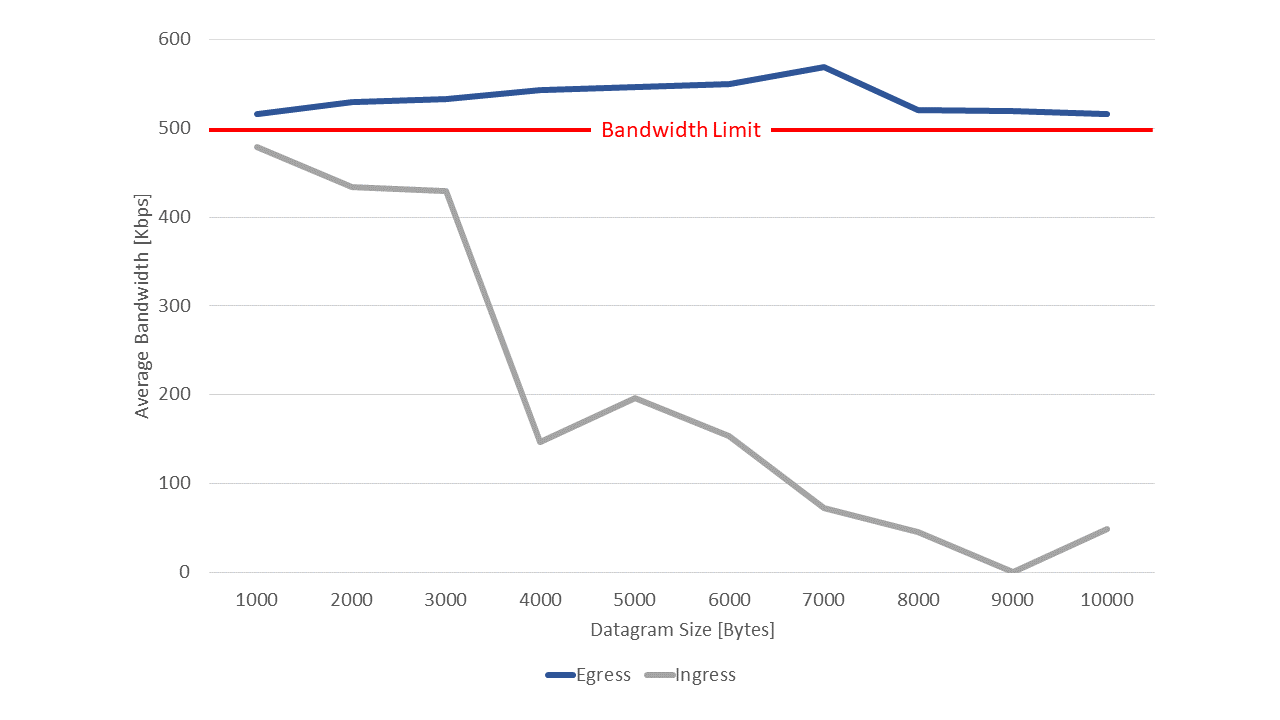
\includegraphics[width=\textwidth]{img/Evaluation-Bandwidth.png}
	\caption{Evaluation of the Bandwidth}
	\label{Evaluation of the Bandwidth}
\end{figure}

\begin{figure}[h]
	\centering
	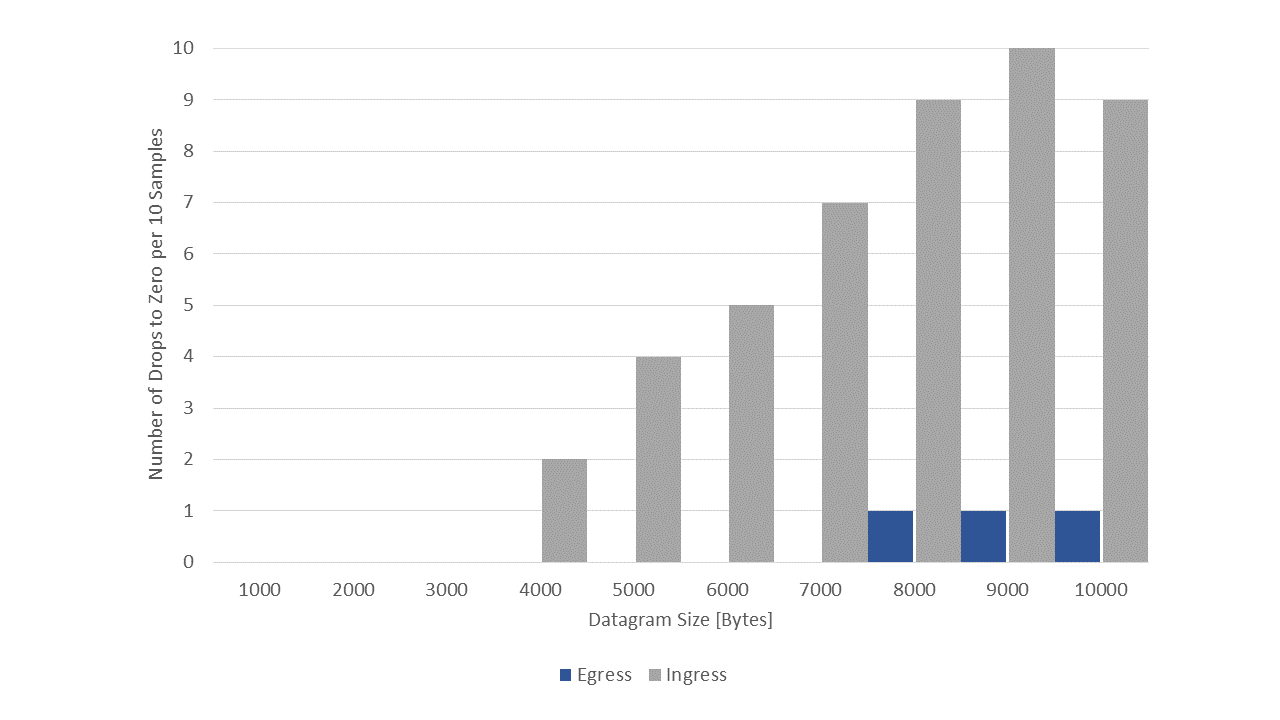
\includegraphics[width=\textwidth]{img/Evaluation-Zeros.png}
	\caption{Evaluation of the Bandwidth Drops}
	\label{Evaluation of the Bandwidth Drops}
\end{figure}

\subsection{Egress Traffic}



\subsection{Ingress Traffic}


%Note: 
%Ingress test: iperf3 -c 192.168.17.129 -u -b 2Mbit -l 1000 -R
%Egress test: iperf3 -c 192.168.17.129 -u -b 2Mbit -l 1000
%important is the -l option that defines the buffer size (KB). otherwise ingress traffic will have one initial burst and then drop to 0

%https://github.com/esnet/iperf/issues/457